% Graphic for TeX using PGF
% Title: /home/guillaume/Documents/Université de Montréal/Automne 2014/Génie logiciel/Devoir/devoir-3/diagramme-de-classes-b.dia
% Creator: Dia v0.97.3
% CreationDate: Sun Dec  7 16:07:22 2014
% For: guillaume
% \usepackage{tikz}
% The following commands are not supported in PSTricks at present
% We define them conditionally, so when they are implemented,
% this pgf file will use them.
\ifx\du\undefined
  \newlength{\du}
\fi
\setlength{\du}{15\unitlength}
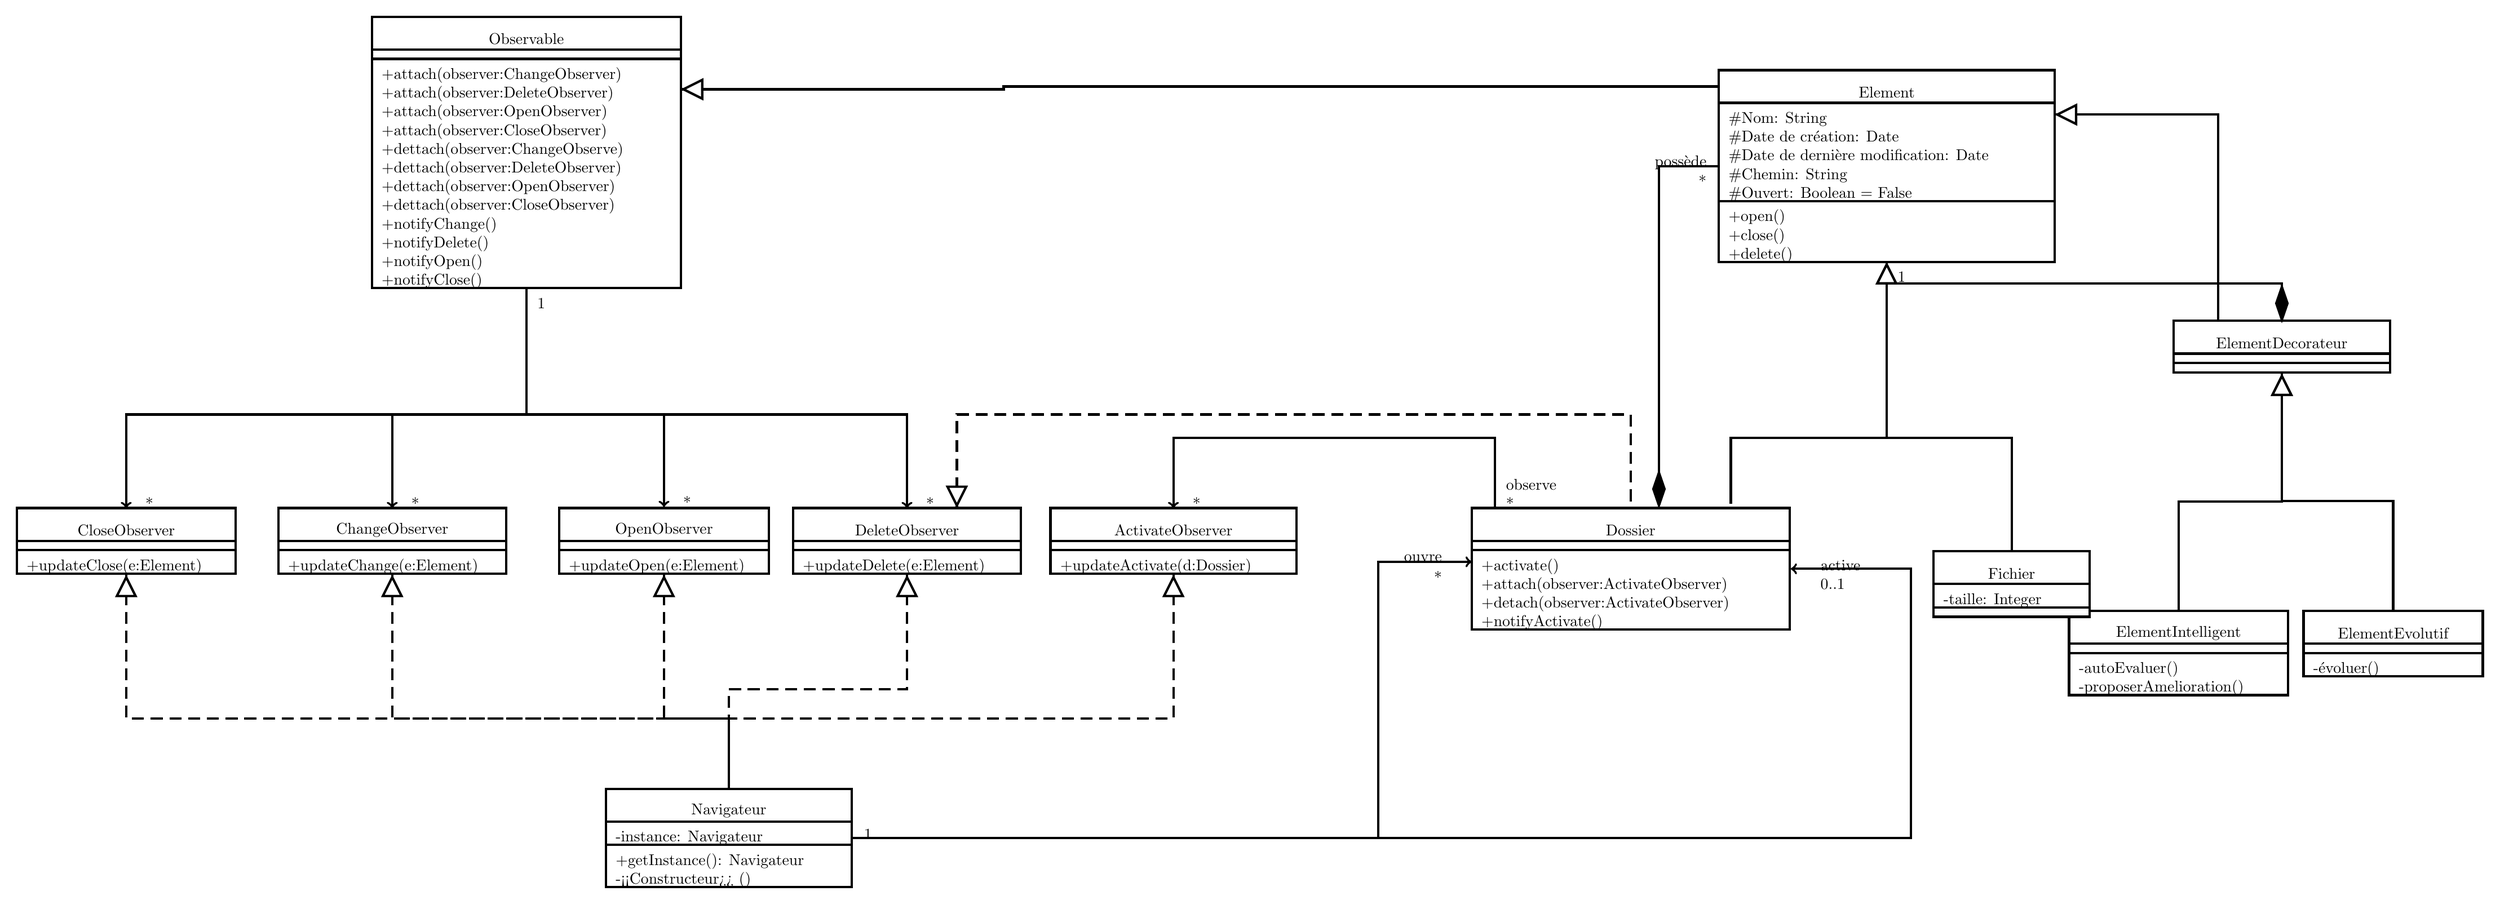
\begin{tikzpicture}
\pgftransformxscale{1.000000}
\pgftransformyscale{-1.000000}
\definecolor{dialinecolor}{rgb}{0.000000, 0.000000, 0.000000}
\pgfsetstrokecolor{dialinecolor}
\definecolor{dialinecolor}{rgb}{1.000000, 1.000000, 1.000000}
\pgfsetfillcolor{dialinecolor}
\pgfsetlinewidth{0.100000\du}
\pgfsetdash{}{0pt}
\definecolor{dialinecolor}{rgb}{1.000000, 1.000000, 1.000000}
\pgfsetfillcolor{dialinecolor}
\fill (23.000000\du,5.000000\du)--(23.000000\du,6.400000\du)--(32.250000\du,6.400000\du)--(32.250000\du,5.000000\du)--cycle;
\definecolor{dialinecolor}{rgb}{0.000000, 0.000000, 0.000000}
\pgfsetstrokecolor{dialinecolor}
\draw (23.000000\du,5.000000\du)--(23.000000\du,6.400000\du)--(32.250000\du,6.400000\du)--(32.250000\du,5.000000\du)--cycle;
% setfont left to latex
\definecolor{dialinecolor}{rgb}{0.000000, 0.000000, 0.000000}
\pgfsetstrokecolor{dialinecolor}
\node at (27.625000\du,5.950000\du){ElementDecorateur};
\definecolor{dialinecolor}{rgb}{1.000000, 1.000000, 1.000000}
\pgfsetfillcolor{dialinecolor}
\fill (23.000000\du,6.400000\du)--(23.000000\du,6.800000\du)--(32.250000\du,6.800000\du)--(32.250000\du,6.400000\du)--cycle;
\definecolor{dialinecolor}{rgb}{0.000000, 0.000000, 0.000000}
\pgfsetstrokecolor{dialinecolor}
\draw (23.000000\du,6.400000\du)--(23.000000\du,6.800000\du)--(32.250000\du,6.800000\du)--(32.250000\du,6.400000\du)--cycle;
\definecolor{dialinecolor}{rgb}{1.000000, 1.000000, 1.000000}
\pgfsetfillcolor{dialinecolor}
\fill (23.000000\du,6.800000\du)--(23.000000\du,7.200000\du)--(32.250000\du,7.200000\du)--(32.250000\du,6.800000\du)--cycle;
\definecolor{dialinecolor}{rgb}{0.000000, 0.000000, 0.000000}
\pgfsetstrokecolor{dialinecolor}
\draw (23.000000\du,6.800000\du)--(23.000000\du,7.200000\du)--(32.250000\du,7.200000\du)--(32.250000\du,6.800000\du)--cycle;
\pgfsetlinewidth{0.100000\du}
\pgfsetdash{}{0pt}
\pgfsetmiterjoin
\pgfsetbuttcap
{
\definecolor{dialinecolor}{rgb}{0.000000, 0.000000, 0.000000}
\pgfsetfillcolor{dialinecolor}
% was here!!!
\definecolor{dialinecolor}{rgb}{0.000000, 0.000000, 0.000000}
\pgfsetstrokecolor{dialinecolor}
\draw (27.625000\du,4.949719\du)--(27.625000\du,3.390596\du)--(10.737700\du,3.390596\du)--(10.737700\du,2.531473\du);
}
\definecolor{dialinecolor}{rgb}{0.000000, 0.000000, 0.000000}
\pgfsetstrokecolor{dialinecolor}
\draw (27.625000\du,3.691141\du)--(27.625000\du,3.390596\du)--(10.737700\du,3.390596\du)--(10.737700\du,2.531473\du);
\pgfsetdash{}{0pt}
\pgfsetmiterjoin
\pgfsetbuttcap
\definecolor{dialinecolor}{rgb}{0.000000, 0.000000, 0.000000}
\pgfsetfillcolor{dialinecolor}
\fill (27.625000\du,4.949719\du)--(27.385000\du,4.249719\du)--(27.625000\du,3.549719\du)--(27.865000\du,4.249719\du)--cycle;
\pgfsetlinewidth{0.100000\du}
\pgfsetdash{}{0pt}
\pgfsetmiterjoin
\pgfsetbuttcap
\definecolor{dialinecolor}{rgb}{0.000000, 0.000000, 0.000000}
\pgfsetstrokecolor{dialinecolor}
\draw (27.625000\du,4.949719\du)--(27.385000\du,4.249719\du)--(27.625000\du,3.549719\du)--(27.865000\du,4.249719\du)--cycle;
% setfont left to latex
\definecolor{dialinecolor}{rgb}{0.000000, 0.000000, 0.000000}
\pgfsetstrokecolor{dialinecolor}
\node at (19.181350\du,3.240596\du){};
\definecolor{dialinecolor}{rgb}{0.000000, 0.000000, 0.000000}
\pgfsetstrokecolor{dialinecolor}
\node[anchor=west] at (28.175000\du,4.749719\du){};
\definecolor{dialinecolor}{rgb}{0.000000, 0.000000, 0.000000}
\pgfsetstrokecolor{dialinecolor}
\node[anchor=west] at (10.937700\du,3.131473\du){1};
\pgfsetlinewidth{0.100000\du}
\pgfsetdash{}{0pt}
\definecolor{dialinecolor}{rgb}{1.000000, 1.000000, 1.000000}
\pgfsetfillcolor{dialinecolor}
\fill (18.531200\du,17.397200\du)--(18.531200\du,18.797200\du)--(27.886200\du,18.797200\du)--(27.886200\du,17.397200\du)--cycle;
\definecolor{dialinecolor}{rgb}{0.000000, 0.000000, 0.000000}
\pgfsetstrokecolor{dialinecolor}
\draw (18.531200\du,17.397200\du)--(18.531200\du,18.797200\du)--(27.886200\du,18.797200\du)--(27.886200\du,17.397200\du)--cycle;
% setfont left to latex
\definecolor{dialinecolor}{rgb}{0.000000, 0.000000, 0.000000}
\pgfsetstrokecolor{dialinecolor}
\node at (23.208700\du,18.347200\du){ElementIntelligent};
\definecolor{dialinecolor}{rgb}{1.000000, 1.000000, 1.000000}
\pgfsetfillcolor{dialinecolor}
\fill (18.531200\du,18.797200\du)--(18.531200\du,19.197200\du)--(27.886200\du,19.197200\du)--(27.886200\du,18.797200\du)--cycle;
\definecolor{dialinecolor}{rgb}{0.000000, 0.000000, 0.000000}
\pgfsetstrokecolor{dialinecolor}
\draw (18.531200\du,18.797200\du)--(18.531200\du,19.197200\du)--(27.886200\du,19.197200\du)--(27.886200\du,18.797200\du)--cycle;
\definecolor{dialinecolor}{rgb}{1.000000, 1.000000, 1.000000}
\pgfsetfillcolor{dialinecolor}
\fill (18.531200\du,19.197200\du)--(18.531200\du,20.997200\du)--(27.886200\du,20.997200\du)--(27.886200\du,19.197200\du)--cycle;
\definecolor{dialinecolor}{rgb}{0.000000, 0.000000, 0.000000}
\pgfsetstrokecolor{dialinecolor}
\draw (18.531200\du,19.197200\du)--(18.531200\du,20.997200\du)--(27.886200\du,20.997200\du)--(27.886200\du,19.197200\du)--cycle;
% setfont left to latex
\definecolor{dialinecolor}{rgb}{0.000000, 0.000000, 0.000000}
\pgfsetstrokecolor{dialinecolor}
\node[anchor=west] at (18.681200\du,19.897200\du){-autoEvaluer()};
% setfont left to latex
\definecolor{dialinecolor}{rgb}{0.000000, 0.000000, 0.000000}
\pgfsetstrokecolor{dialinecolor}
\node[anchor=west] at (18.681200\du,20.697200\du){-proposerAmelioration()};
\pgfsetlinewidth{0.100000\du}
\pgfsetdash{}{0pt}
\definecolor{dialinecolor}{rgb}{1.000000, 1.000000, 1.000000}
\pgfsetfillcolor{dialinecolor}
\fill (28.549900\du,17.397200\du)--(28.549900\du,18.797200\du)--(36.212400\du,18.797200\du)--(36.212400\du,17.397200\du)--cycle;
\definecolor{dialinecolor}{rgb}{0.000000, 0.000000, 0.000000}
\pgfsetstrokecolor{dialinecolor}
\draw (28.549900\du,17.397200\du)--(28.549900\du,18.797200\du)--(36.212400\du,18.797200\du)--(36.212400\du,17.397200\du)--cycle;
% setfont left to latex
\definecolor{dialinecolor}{rgb}{0.000000, 0.000000, 0.000000}
\pgfsetstrokecolor{dialinecolor}
\node at (32.381150\du,18.347200\du){ElementEvolutif};
\definecolor{dialinecolor}{rgb}{1.000000, 1.000000, 1.000000}
\pgfsetfillcolor{dialinecolor}
\fill (28.549900\du,18.797200\du)--(28.549900\du,19.197200\du)--(36.212400\du,19.197200\du)--(36.212400\du,18.797200\du)--cycle;
\definecolor{dialinecolor}{rgb}{0.000000, 0.000000, 0.000000}
\pgfsetstrokecolor{dialinecolor}
\draw (28.549900\du,18.797200\du)--(28.549900\du,19.197200\du)--(36.212400\du,19.197200\du)--(36.212400\du,18.797200\du)--cycle;
\definecolor{dialinecolor}{rgb}{1.000000, 1.000000, 1.000000}
\pgfsetfillcolor{dialinecolor}
\fill (28.549900\du,19.197200\du)--(28.549900\du,20.197200\du)--(36.212400\du,20.197200\du)--(36.212400\du,19.197200\du)--cycle;
\definecolor{dialinecolor}{rgb}{0.000000, 0.000000, 0.000000}
\pgfsetstrokecolor{dialinecolor}
\draw (28.549900\du,19.197200\du)--(28.549900\du,20.197200\du)--(36.212400\du,20.197200\du)--(36.212400\du,19.197200\du)--cycle;
% setfont left to latex
\definecolor{dialinecolor}{rgb}{0.000000, 0.000000, 0.000000}
\pgfsetstrokecolor{dialinecolor}
\node[anchor=west] at (28.699900\du,19.897200\du){-évoluer()};
\pgfsetlinewidth{0.100000\du}
\pgfsetdash{}{0pt}
\pgfsetmiterjoin
\pgfsetbuttcap
{
\definecolor{dialinecolor}{rgb}{0.000000, 0.000000, 0.000000}
\pgfsetfillcolor{dialinecolor}
% was here!!!
\definecolor{dialinecolor}{rgb}{0.000000, 0.000000, 0.000000}
\pgfsetstrokecolor{dialinecolor}
\draw (27.625000\du,7.250281\du)--(27.625000\du,12.723740\du)--(23.208700\du,12.723740\du)--(23.208700\du,17.397200\du);
}
\definecolor{dialinecolor}{rgb}{0.000000, 0.000000, 0.000000}
\pgfsetstrokecolor{dialinecolor}
\draw (27.625000\du,8.162084\du)--(27.625000\du,12.723740\du)--(23.208700\du,12.723740\du)--(23.208700\du,17.397200\du);
\pgfsetmiterjoin
\definecolor{dialinecolor}{rgb}{1.000000, 1.000000, 1.000000}
\pgfsetfillcolor{dialinecolor}
\fill (28.025000\du,8.162084\du)--(27.625000\du,7.362084\du)--(27.225000\du,8.162084\du)--cycle;
\pgfsetlinewidth{0.100000\du}
\pgfsetdash{}{0pt}
\pgfsetmiterjoin
\definecolor{dialinecolor}{rgb}{0.000000, 0.000000, 0.000000}
\pgfsetstrokecolor{dialinecolor}
\draw (28.025000\du,8.162084\du)--(27.625000\du,7.362084\du)--(27.225000\du,8.162084\du)--cycle;
% setfont left to latex
\pgfsetlinewidth{0.100000\du}
\pgfsetdash{}{0pt}
\pgfsetmiterjoin
\pgfsetbuttcap
{
\definecolor{dialinecolor}{rgb}{0.000000, 0.000000, 0.000000}
\pgfsetfillcolor{dialinecolor}
% was here!!!
\definecolor{dialinecolor}{rgb}{0.000000, 0.000000, 0.000000}
\pgfsetstrokecolor{dialinecolor}
\draw (27.625000\du,7.250281\du)--(27.625000\du,12.698563\du)--(32.381150\du,12.698563\du)--(32.381150\du,17.346846\du);
}
\definecolor{dialinecolor}{rgb}{0.000000, 0.000000, 0.000000}
\pgfsetstrokecolor{dialinecolor}
\draw (27.625000\du,8.162084\du)--(27.625000\du,12.698563\du)--(32.381150\du,12.698563\du)--(32.381150\du,17.346846\du);
\pgfsetmiterjoin
\definecolor{dialinecolor}{rgb}{1.000000, 1.000000, 1.000000}
\pgfsetfillcolor{dialinecolor}
\fill (28.025000\du,8.162084\du)--(27.625000\du,7.362084\du)--(27.225000\du,8.162084\du)--cycle;
\pgfsetlinewidth{0.100000\du}
\pgfsetdash{}{0pt}
\pgfsetmiterjoin
\definecolor{dialinecolor}{rgb}{0.000000, 0.000000, 0.000000}
\pgfsetstrokecolor{dialinecolor}
\draw (28.025000\du,8.162084\du)--(27.625000\du,7.362084\du)--(27.225000\du,8.162084\du)--cycle;
% setfont left to latex
\pgfsetlinewidth{0.100000\du}
\pgfsetdash{}{0pt}
\pgfsetmiterjoin
\pgfsetbuttcap
{
\definecolor{dialinecolor}{rgb}{0.000000, 0.000000, 0.000000}
\pgfsetfillcolor{dialinecolor}
% was here!!!
\definecolor{dialinecolor}{rgb}{0.000000, 0.000000, 0.000000}
\pgfsetstrokecolor{dialinecolor}
\draw (17.917700\du,-3.818780\du)--(24.892100\du,-3.818780\du)--(24.892100\du,5.000000\du)--(27.142500\du,5.000000\du);
}
\definecolor{dialinecolor}{rgb}{0.000000, 0.000000, 0.000000}
\pgfsetstrokecolor{dialinecolor}
\draw (18.829503\du,-3.818780\du)--(24.892100\du,-3.818780\du)--(24.892100\du,5.000000\du)--(27.142500\du,5.000000\du);
\pgfsetmiterjoin
\definecolor{dialinecolor}{rgb}{1.000000, 1.000000, 1.000000}
\pgfsetfillcolor{dialinecolor}
\fill (18.829503\du,-4.218780\du)--(18.029503\du,-3.818780\du)--(18.829503\du,-3.418780\du)--cycle;
\pgfsetlinewidth{0.100000\du}
\pgfsetdash{}{0pt}
\pgfsetmiterjoin
\definecolor{dialinecolor}{rgb}{0.000000, 0.000000, 0.000000}
\pgfsetstrokecolor{dialinecolor}
\draw (18.829503\du,-4.218780\du)--(18.029503\du,-3.818780\du)--(18.829503\du,-3.418780\du)--cycle;
% setfont left to latex
\pgfsetlinewidth{0.100000\du}
\pgfsetdash{}{0pt}
\definecolor{dialinecolor}{rgb}{1.000000, 1.000000, 1.000000}
\pgfsetfillcolor{dialinecolor}
\fill (3.557700\du,-5.718780\du)--(3.557700\du,-4.318780\du)--(17.917700\du,-4.318780\du)--(17.917700\du,-5.718780\du)--cycle;
\definecolor{dialinecolor}{rgb}{0.000000, 0.000000, 0.000000}
\pgfsetstrokecolor{dialinecolor}
\draw (3.557700\du,-5.718780\du)--(3.557700\du,-4.318780\du)--(17.917700\du,-4.318780\du)--(17.917700\du,-5.718780\du)--cycle;
% setfont left to latex
\definecolor{dialinecolor}{rgb}{0.000000, 0.000000, 0.000000}
\pgfsetstrokecolor{dialinecolor}
\node at (10.737700\du,-4.768780\du){Element};
\definecolor{dialinecolor}{rgb}{1.000000, 1.000000, 1.000000}
\pgfsetfillcolor{dialinecolor}
\fill (3.557700\du,-4.318780\du)--(3.557700\du,-0.118780\du)--(17.917700\du,-0.118780\du)--(17.917700\du,-4.318780\du)--cycle;
\definecolor{dialinecolor}{rgb}{0.000000, 0.000000, 0.000000}
\pgfsetstrokecolor{dialinecolor}
\draw (3.557700\du,-4.318780\du)--(3.557700\du,-0.118780\du)--(17.917700\du,-0.118780\du)--(17.917700\du,-4.318780\du)--cycle;
% setfont left to latex
\definecolor{dialinecolor}{rgb}{0.000000, 0.000000, 0.000000}
\pgfsetstrokecolor{dialinecolor}
\node[anchor=west] at (3.707700\du,-3.618780\du){\#Nom: String};
% setfont left to latex
\definecolor{dialinecolor}{rgb}{0.000000, 0.000000, 0.000000}
\pgfsetstrokecolor{dialinecolor}
\node[anchor=west] at (3.707700\du,-2.818780\du){\#Date de création: Date};
% setfont left to latex
\definecolor{dialinecolor}{rgb}{0.000000, 0.000000, 0.000000}
\pgfsetstrokecolor{dialinecolor}
\node[anchor=west] at (3.707700\du,-2.018780\du){\#Date de dernière modification: Date};
% setfont left to latex
\definecolor{dialinecolor}{rgb}{0.000000, 0.000000, 0.000000}
\pgfsetstrokecolor{dialinecolor}
\node[anchor=west] at (3.707700\du,-1.218780\du){\#Chemin: String};
% setfont left to latex
\definecolor{dialinecolor}{rgb}{0.000000, 0.000000, 0.000000}
\pgfsetstrokecolor{dialinecolor}
\node[anchor=west] at (3.707700\du,-0.418780\du){\#Ouvert: Boolean = False};
\definecolor{dialinecolor}{rgb}{1.000000, 1.000000, 1.000000}
\pgfsetfillcolor{dialinecolor}
\fill (3.557700\du,-0.118780\du)--(3.557700\du,2.481220\du)--(17.917700\du,2.481220\du)--(17.917700\du,-0.118780\du)--cycle;
\definecolor{dialinecolor}{rgb}{0.000000, 0.000000, 0.000000}
\pgfsetstrokecolor{dialinecolor}
\draw (3.557700\du,-0.118780\du)--(3.557700\du,2.481220\du)--(17.917700\du,2.481220\du)--(17.917700\du,-0.118780\du)--cycle;
% setfont left to latex
\definecolor{dialinecolor}{rgb}{0.000000, 0.000000, 0.000000}
\pgfsetstrokecolor{dialinecolor}
\node[anchor=west] at (3.707700\du,0.581220\du){+open()};
% setfont left to latex
\definecolor{dialinecolor}{rgb}{0.000000, 0.000000, 0.000000}
\pgfsetstrokecolor{dialinecolor}
\node[anchor=west] at (3.707700\du,1.381220\du){+close()};
% setfont left to latex
\definecolor{dialinecolor}{rgb}{0.000000, 0.000000, 0.000000}
\pgfsetstrokecolor{dialinecolor}
\node[anchor=west] at (3.707700\du,2.181220\du){+delete()};
\pgfsetlinewidth{0.100000\du}
\pgfsetdash{}{0pt}
\definecolor{dialinecolor}{rgb}{1.000000, 1.000000, 1.000000}
\pgfsetfillcolor{dialinecolor}
\fill (12.745400\du,14.848800\du)--(12.745400\du,16.248800\du)--(19.405400\du,16.248800\du)--(19.405400\du,14.848800\du)--cycle;
\definecolor{dialinecolor}{rgb}{0.000000, 0.000000, 0.000000}
\pgfsetstrokecolor{dialinecolor}
\draw (12.745400\du,14.848800\du)--(12.745400\du,16.248800\du)--(19.405400\du,16.248800\du)--(19.405400\du,14.848800\du)--cycle;
% setfont left to latex
\definecolor{dialinecolor}{rgb}{0.000000, 0.000000, 0.000000}
\pgfsetstrokecolor{dialinecolor}
\node at (16.075400\du,15.798800\du){Fichier};
\definecolor{dialinecolor}{rgb}{1.000000, 1.000000, 1.000000}
\pgfsetfillcolor{dialinecolor}
\fill (12.745400\du,16.248800\du)--(12.745400\du,17.248800\du)--(19.405400\du,17.248800\du)--(19.405400\du,16.248800\du)--cycle;
\definecolor{dialinecolor}{rgb}{0.000000, 0.000000, 0.000000}
\pgfsetstrokecolor{dialinecolor}
\draw (12.745400\du,16.248800\du)--(12.745400\du,17.248800\du)--(19.405400\du,17.248800\du)--(19.405400\du,16.248800\du)--cycle;
% setfont left to latex
\definecolor{dialinecolor}{rgb}{0.000000, 0.000000, 0.000000}
\pgfsetstrokecolor{dialinecolor}
\node[anchor=west] at (12.895400\du,16.948800\du){-taille: Integer};
\definecolor{dialinecolor}{rgb}{1.000000, 1.000000, 1.000000}
\pgfsetfillcolor{dialinecolor}
\fill (12.745400\du,17.248800\du)--(12.745400\du,17.648800\du)--(19.405400\du,17.648800\du)--(19.405400\du,17.248800\du)--cycle;
\definecolor{dialinecolor}{rgb}{0.000000, 0.000000, 0.000000}
\pgfsetstrokecolor{dialinecolor}
\draw (12.745400\du,17.248800\du)--(12.745400\du,17.648800\du)--(19.405400\du,17.648800\du)--(19.405400\du,17.248800\du)--cycle;
\pgfsetlinewidth{0.100000\du}
\pgfsetdash{}{0pt}
\definecolor{dialinecolor}{rgb}{1.000000, 1.000000, 1.000000}
\pgfsetfillcolor{dialinecolor}
\fill (-7.000000\du,13.000000\du)--(-7.000000\du,14.400000\du)--(6.590000\du,14.400000\du)--(6.590000\du,13.000000\du)--cycle;
\definecolor{dialinecolor}{rgb}{0.000000, 0.000000, 0.000000}
\pgfsetstrokecolor{dialinecolor}
\draw (-7.000000\du,13.000000\du)--(-7.000000\du,14.400000\du)--(6.590000\du,14.400000\du)--(6.590000\du,13.000000\du)--cycle;
% setfont left to latex
\definecolor{dialinecolor}{rgb}{0.000000, 0.000000, 0.000000}
\pgfsetstrokecolor{dialinecolor}
\node at (-0.205000\du,13.950000\du){Dossier};
\definecolor{dialinecolor}{rgb}{1.000000, 1.000000, 1.000000}
\pgfsetfillcolor{dialinecolor}
\fill (-7.000000\du,14.400000\du)--(-7.000000\du,14.800000\du)--(6.590000\du,14.800000\du)--(6.590000\du,14.400000\du)--cycle;
\definecolor{dialinecolor}{rgb}{0.000000, 0.000000, 0.000000}
\pgfsetstrokecolor{dialinecolor}
\draw (-7.000000\du,14.400000\du)--(-7.000000\du,14.800000\du)--(6.590000\du,14.800000\du)--(6.590000\du,14.400000\du)--cycle;
\definecolor{dialinecolor}{rgb}{1.000000, 1.000000, 1.000000}
\pgfsetfillcolor{dialinecolor}
\fill (-7.000000\du,14.800000\du)--(-7.000000\du,18.200000\du)--(6.590000\du,18.200000\du)--(6.590000\du,14.800000\du)--cycle;
\definecolor{dialinecolor}{rgb}{0.000000, 0.000000, 0.000000}
\pgfsetstrokecolor{dialinecolor}
\draw (-7.000000\du,14.800000\du)--(-7.000000\du,18.200000\du)--(6.590000\du,18.200000\du)--(6.590000\du,14.800000\du)--cycle;
% setfont left to latex
\definecolor{dialinecolor}{rgb}{0.000000, 0.000000, 0.000000}
\pgfsetstrokecolor{dialinecolor}
\node[anchor=west] at (-6.850000\du,15.500000\du){+activate()};
% setfont left to latex
\definecolor{dialinecolor}{rgb}{0.000000, 0.000000, 0.000000}
\pgfsetstrokecolor{dialinecolor}
\node[anchor=west] at (-6.850000\du,16.300000\du){+attach(observer:ActivateObserver)};
% setfont left to latex
\definecolor{dialinecolor}{rgb}{0.000000, 0.000000, 0.000000}
\pgfsetstrokecolor{dialinecolor}
\node[anchor=west] at (-6.850000\du,17.100000\du){+detach(observer:ActivateObserver)};
% setfont left to latex
\definecolor{dialinecolor}{rgb}{0.000000, 0.000000, 0.000000}
\pgfsetstrokecolor{dialinecolor}
\node[anchor=west] at (-6.850000\du,17.900000\du){+notifyActivate()};
\pgfsetlinewidth{0.100000\du}
\pgfsetdash{}{0pt}
\definecolor{dialinecolor}{rgb}{1.000000, 1.000000, 1.000000}
\pgfsetfillcolor{dialinecolor}
\fill (-44.000000\du,25.000000\du)--(-44.000000\du,26.400000\du)--(-33.490000\du,26.400000\du)--(-33.490000\du,25.000000\du)--cycle;
\definecolor{dialinecolor}{rgb}{0.000000, 0.000000, 0.000000}
\pgfsetstrokecolor{dialinecolor}
\draw (-44.000000\du,25.000000\du)--(-44.000000\du,26.400000\du)--(-33.490000\du,26.400000\du)--(-33.490000\du,25.000000\du)--cycle;
% setfont left to latex
\definecolor{dialinecolor}{rgb}{0.000000, 0.000000, 0.000000}
\pgfsetstrokecolor{dialinecolor}
\node at (-38.745000\du,25.950000\du){Navigateur};
\definecolor{dialinecolor}{rgb}{1.000000, 1.000000, 1.000000}
\pgfsetfillcolor{dialinecolor}
\fill (-44.000000\du,26.400000\du)--(-44.000000\du,27.400000\du)--(-33.490000\du,27.400000\du)--(-33.490000\du,26.400000\du)--cycle;
\definecolor{dialinecolor}{rgb}{0.000000, 0.000000, 0.000000}
\pgfsetstrokecolor{dialinecolor}
\draw (-44.000000\du,26.400000\du)--(-44.000000\du,27.400000\du)--(-33.490000\du,27.400000\du)--(-33.490000\du,26.400000\du)--cycle;
% setfont left to latex
\definecolor{dialinecolor}{rgb}{0.000000, 0.000000, 0.000000}
\pgfsetstrokecolor{dialinecolor}
\node[anchor=west] at (-43.850000\du,27.100000\du){-instance: Navigateur};
\definecolor{dialinecolor}{rgb}{1.000000, 1.000000, 1.000000}
\pgfsetfillcolor{dialinecolor}
\fill (-44.000000\du,27.400000\du)--(-44.000000\du,29.200000\du)--(-33.490000\du,29.200000\du)--(-33.490000\du,27.400000\du)--cycle;
\definecolor{dialinecolor}{rgb}{0.000000, 0.000000, 0.000000}
\pgfsetstrokecolor{dialinecolor}
\draw (-44.000000\du,27.400000\du)--(-44.000000\du,29.200000\du)--(-33.490000\du,29.200000\du)--(-33.490000\du,27.400000\du)--cycle;
% setfont left to latex
\definecolor{dialinecolor}{rgb}{0.000000, 0.000000, 0.000000}
\pgfsetstrokecolor{dialinecolor}
\node[anchor=west] at (-43.850000\du,28.100000\du){+getInstance(): Navigateur};
% setfont left to latex
\definecolor{dialinecolor}{rgb}{0.000000, 0.000000, 0.000000}
\pgfsetstrokecolor{dialinecolor}
\node[anchor=west] at (-43.850000\du,28.900000\du){-<<Constructeur>> ()};
\pgfsetlinewidth{0.100000\du}
\pgfsetdash{}{0pt}
\pgfsetmiterjoin
\pgfsetbuttcap
{
\definecolor{dialinecolor}{rgb}{0.000000, 0.000000, 0.000000}
\pgfsetfillcolor{dialinecolor}
% was here!!!
\definecolor{dialinecolor}{rgb}{0.000000, 0.000000, 0.000000}
\pgfsetstrokecolor{dialinecolor}
\draw (10.737700\du,2.481220\du)--(10.737700\du,10.000000\du)--(4.076380\du,10.000000\du)--(4.076380\du,12.809900\du);
}
\definecolor{dialinecolor}{rgb}{0.000000, 0.000000, 0.000000}
\pgfsetstrokecolor{dialinecolor}
\draw (10.737700\du,3.393023\du)--(10.737700\du,10.000000\du)--(4.076380\du,10.000000\du)--(4.076380\du,12.809900\du);
\pgfsetmiterjoin
\definecolor{dialinecolor}{rgb}{1.000000, 1.000000, 1.000000}
\pgfsetfillcolor{dialinecolor}
\fill (11.137700\du,3.393023\du)--(10.737700\du,2.593023\du)--(10.337700\du,3.393023\du)--cycle;
\pgfsetlinewidth{0.100000\du}
\pgfsetdash{}{0pt}
\pgfsetmiterjoin
\definecolor{dialinecolor}{rgb}{0.000000, 0.000000, 0.000000}
\pgfsetstrokecolor{dialinecolor}
\draw (11.137700\du,3.393023\du)--(10.737700\du,2.593023\du)--(10.337700\du,3.393023\du)--cycle;
% setfont left to latex
\pgfsetlinewidth{0.100000\du}
\pgfsetdash{}{0pt}
\pgfsetmiterjoin
\pgfsetbuttcap
{
\definecolor{dialinecolor}{rgb}{0.000000, 0.000000, 0.000000}
\pgfsetfillcolor{dialinecolor}
% was here!!!
\definecolor{dialinecolor}{rgb}{0.000000, 0.000000, 0.000000}
\pgfsetstrokecolor{dialinecolor}
\draw (10.737700\du,2.481220\du)--(10.737700\du,10.000000\du)--(16.075400\du,10.000000\du)--(16.075400\du,14.798731\du);
}
\definecolor{dialinecolor}{rgb}{0.000000, 0.000000, 0.000000}
\pgfsetstrokecolor{dialinecolor}
\draw (10.737700\du,3.393023\du)--(10.737700\du,10.000000\du)--(16.075400\du,10.000000\du)--(16.075400\du,14.798731\du);
\pgfsetmiterjoin
\definecolor{dialinecolor}{rgb}{1.000000, 1.000000, 1.000000}
\pgfsetfillcolor{dialinecolor}
\fill (11.137700\du,3.393023\du)--(10.737700\du,2.593023\du)--(10.337700\du,3.393023\du)--cycle;
\pgfsetlinewidth{0.100000\du}
\pgfsetdash{}{0pt}
\pgfsetmiterjoin
\definecolor{dialinecolor}{rgb}{0.000000, 0.000000, 0.000000}
\pgfsetstrokecolor{dialinecolor}
\draw (11.137700\du,3.393023\du)--(10.737700\du,2.593023\du)--(10.337700\du,3.393023\du)--cycle;
% setfont left to latex
\pgfsetlinewidth{0.100000\du}
\pgfsetdash{}{0pt}
\definecolor{dialinecolor}{rgb}{1.000000, 1.000000, 1.000000}
\pgfsetfillcolor{dialinecolor}
\fill (-54.000000\du,-8.000000\du)--(-54.000000\du,-6.600000\du)--(-40.795000\du,-6.600000\du)--(-40.795000\du,-8.000000\du)--cycle;
\definecolor{dialinecolor}{rgb}{0.000000, 0.000000, 0.000000}
\pgfsetstrokecolor{dialinecolor}
\draw (-54.000000\du,-8.000000\du)--(-54.000000\du,-6.600000\du)--(-40.795000\du,-6.600000\du)--(-40.795000\du,-8.000000\du)--cycle;
% setfont left to latex
\definecolor{dialinecolor}{rgb}{0.000000, 0.000000, 0.000000}
\pgfsetstrokecolor{dialinecolor}
\node at (-47.397500\du,-7.050000\du){Observable};
\definecolor{dialinecolor}{rgb}{1.000000, 1.000000, 1.000000}
\pgfsetfillcolor{dialinecolor}
\fill (-54.000000\du,-6.600000\du)--(-54.000000\du,-6.200000\du)--(-40.795000\du,-6.200000\du)--(-40.795000\du,-6.600000\du)--cycle;
\definecolor{dialinecolor}{rgb}{0.000000, 0.000000, 0.000000}
\pgfsetstrokecolor{dialinecolor}
\draw (-54.000000\du,-6.600000\du)--(-54.000000\du,-6.200000\du)--(-40.795000\du,-6.200000\du)--(-40.795000\du,-6.600000\du)--cycle;
\definecolor{dialinecolor}{rgb}{1.000000, 1.000000, 1.000000}
\pgfsetfillcolor{dialinecolor}
\fill (-54.000000\du,-6.200000\du)--(-54.000000\du,3.600000\du)--(-40.795000\du,3.600000\du)--(-40.795000\du,-6.200000\du)--cycle;
\definecolor{dialinecolor}{rgb}{0.000000, 0.000000, 0.000000}
\pgfsetstrokecolor{dialinecolor}
\draw (-54.000000\du,-6.200000\du)--(-54.000000\du,3.600000\du)--(-40.795000\du,3.600000\du)--(-40.795000\du,-6.200000\du)--cycle;
% setfont left to latex
\definecolor{dialinecolor}{rgb}{0.000000, 0.000000, 0.000000}
\pgfsetstrokecolor{dialinecolor}
\node[anchor=west] at (-53.850000\du,-5.500000\du){+attach(observer:ChangeObserver)};
% setfont left to latex
\definecolor{dialinecolor}{rgb}{0.000000, 0.000000, 0.000000}
\pgfsetstrokecolor{dialinecolor}
\node[anchor=west] at (-53.850000\du,-4.700000\du){+attach(observer:DeleteObserver)};
% setfont left to latex
\definecolor{dialinecolor}{rgb}{0.000000, 0.000000, 0.000000}
\pgfsetstrokecolor{dialinecolor}
\node[anchor=west] at (-53.850000\du,-3.900000\du){+attach(observer:OpenObserver)};
% setfont left to latex
\definecolor{dialinecolor}{rgb}{0.000000, 0.000000, 0.000000}
\pgfsetstrokecolor{dialinecolor}
\node[anchor=west] at (-53.850000\du,-3.100000\du){+attach(observer:CloseObserver)};
% setfont left to latex
\definecolor{dialinecolor}{rgb}{0.000000, 0.000000, 0.000000}
\pgfsetstrokecolor{dialinecolor}
\node[anchor=west] at (-53.850000\du,-2.300000\du){+dettach(observer:ChangeObserve)};
% setfont left to latex
\definecolor{dialinecolor}{rgb}{0.000000, 0.000000, 0.000000}
\pgfsetstrokecolor{dialinecolor}
\node[anchor=west] at (-53.850000\du,-1.500000\du){+dettach(observer:DeleteObserver)};
% setfont left to latex
\definecolor{dialinecolor}{rgb}{0.000000, 0.000000, 0.000000}
\pgfsetstrokecolor{dialinecolor}
\node[anchor=west] at (-53.850000\du,-0.700000\du){+dettach(observer:OpenObserver)};
% setfont left to latex
\definecolor{dialinecolor}{rgb}{0.000000, 0.000000, 0.000000}
\pgfsetstrokecolor{dialinecolor}
\node[anchor=west] at (-53.850000\du,0.100000\du){+dettach(observer:CloseObserver)};
% setfont left to latex
\definecolor{dialinecolor}{rgb}{0.000000, 0.000000, 0.000000}
\pgfsetstrokecolor{dialinecolor}
\node[anchor=west] at (-53.850000\du,0.900000\du){+notifyChange()};
% setfont left to latex
\definecolor{dialinecolor}{rgb}{0.000000, 0.000000, 0.000000}
\pgfsetstrokecolor{dialinecolor}
\node[anchor=west] at (-53.850000\du,1.700000\du){+notifyDelete()};
% setfont left to latex
\definecolor{dialinecolor}{rgb}{0.000000, 0.000000, 0.000000}
\pgfsetstrokecolor{dialinecolor}
\node[anchor=west] at (-53.850000\du,2.500000\du){+notifyOpen()};
% setfont left to latex
\definecolor{dialinecolor}{rgb}{0.000000, 0.000000, 0.000000}
\pgfsetstrokecolor{dialinecolor}
\node[anchor=west] at (-53.850000\du,3.300000\du){+notifyClose()};
\pgfsetlinewidth{0.100000\du}
\pgfsetdash{}{0pt}
\pgfsetmiterjoin
\pgfsetbuttcap
{
\definecolor{dialinecolor}{rgb}{0.000000, 0.000000, 0.000000}
\pgfsetfillcolor{dialinecolor}
% was here!!!
\definecolor{dialinecolor}{rgb}{0.000000, 0.000000, 0.000000}
\pgfsetstrokecolor{dialinecolor}
\draw (1.003770\du,12.886700\du)--(1.003770\du,12.886700\du)--(1.003770\du,-1.618780\du)--(3.507952\du,-1.618780\du);
}
\definecolor{dialinecolor}{rgb}{0.000000, 0.000000, 0.000000}
\pgfsetstrokecolor{dialinecolor}
\draw (1.003770\du,11.628121\du)--(1.003770\du,-1.618780\du)--(3.507952\du,-1.618780\du);
\pgfsetdash{}{0pt}
\pgfsetmiterjoin
\pgfsetbuttcap
\definecolor{dialinecolor}{rgb}{0.000000, 0.000000, 0.000000}
\pgfsetfillcolor{dialinecolor}
\fill (1.003770\du,12.886700\du)--(0.763770\du,12.186700\du)--(1.003770\du,11.486700\du)--(1.243770\du,12.186700\du)--cycle;
\pgfsetlinewidth{0.100000\du}
\pgfsetdash{}{0pt}
\pgfsetmiterjoin
\pgfsetbuttcap
\definecolor{dialinecolor}{rgb}{0.000000, 0.000000, 0.000000}
\pgfsetstrokecolor{dialinecolor}
\draw (1.003770\du,12.886700\du)--(0.763770\du,12.186700\du)--(1.003770\du,11.486700\du)--(1.243770\du,12.186700\du)--cycle;
% setfont left to latex
\definecolor{dialinecolor}{rgb}{0.000000, 0.000000, 0.000000}
\pgfsetstrokecolor{dialinecolor}
\node[anchor=west] at (1.103770\du,5.483960\du){};
\definecolor{dialinecolor}{rgb}{0.000000, 0.000000, 0.000000}
\pgfsetstrokecolor{dialinecolor}
\node[anchor=west] at (1.553770\du,12.686700\du){};
\definecolor{dialinecolor}{rgb}{0.000000, 0.000000, 0.000000}
\pgfsetstrokecolor{dialinecolor}
\node[anchor=east] at (3.307952\du,-1.768780\du){ possède};
\definecolor{dialinecolor}{rgb}{0.000000, 0.000000, 0.000000}
\pgfsetstrokecolor{dialinecolor}
\node[anchor=east] at (3.307952\du,-0.968780\du){*};
\pgfsetlinewidth{0.100000\du}
\pgfsetdash{}{0pt}
\pgfsetmiterjoin
\pgfsetbuttcap
{
\definecolor{dialinecolor}{rgb}{0.000000, 0.000000, 0.000000}
\pgfsetfillcolor{dialinecolor}
% was here!!!
\pgfsetarrowsend{to}
\definecolor{dialinecolor}{rgb}{0.000000, 0.000000, 0.000000}
\pgfsetstrokecolor{dialinecolor}
\draw (-33.440616\du,27.100000\du)--(11.775000\du,27.100000\du)--(11.775000\du,15.600000\du)--(6.639774\du,15.600000\du);
}
% setfont left to latex
\definecolor{dialinecolor}{rgb}{0.000000, 0.000000, 0.000000}
\pgfsetstrokecolor{dialinecolor}
\node[anchor=west] at (11.875000\du,21.200000\du){};
\definecolor{dialinecolor}{rgb}{0.000000, 0.000000, 0.000000}
\pgfsetstrokecolor{dialinecolor}
\node[anchor=west] at (-33.240616\du,26.950000\du){};
\definecolor{dialinecolor}{rgb}{0.000000, 0.000000, 0.000000}
\pgfsetstrokecolor{dialinecolor}
\node[anchor=west] at (7.639774\du,15.450000\du){ active};
\definecolor{dialinecolor}{rgb}{0.000000, 0.000000, 0.000000}
\pgfsetstrokecolor{dialinecolor}
\node[anchor=west] at (7.639774\du,16.250000\du){0..1};
\pgfsetlinewidth{0.100000\du}
\pgfsetdash{}{0pt}
\definecolor{dialinecolor}{rgb}{1.000000, 1.000000, 1.000000}
\pgfsetfillcolor{dialinecolor}
\fill (-25.000000\du,13.000000\du)--(-25.000000\du,14.400000\du)--(-14.490000\du,14.400000\du)--(-14.490000\du,13.000000\du)--cycle;
\definecolor{dialinecolor}{rgb}{0.000000, 0.000000, 0.000000}
\pgfsetstrokecolor{dialinecolor}
\draw (-25.000000\du,13.000000\du)--(-25.000000\du,14.400000\du)--(-14.490000\du,14.400000\du)--(-14.490000\du,13.000000\du)--cycle;
% setfont left to latex
\definecolor{dialinecolor}{rgb}{0.000000, 0.000000, 0.000000}
\pgfsetstrokecolor{dialinecolor}
\node at (-19.745000\du,13.950000\du){ActivateObserver};
\definecolor{dialinecolor}{rgb}{1.000000, 1.000000, 1.000000}
\pgfsetfillcolor{dialinecolor}
\fill (-25.000000\du,14.400000\du)--(-25.000000\du,14.800000\du)--(-14.490000\du,14.800000\du)--(-14.490000\du,14.400000\du)--cycle;
\definecolor{dialinecolor}{rgb}{0.000000, 0.000000, 0.000000}
\pgfsetstrokecolor{dialinecolor}
\draw (-25.000000\du,14.400000\du)--(-25.000000\du,14.800000\du)--(-14.490000\du,14.800000\du)--(-14.490000\du,14.400000\du)--cycle;
\definecolor{dialinecolor}{rgb}{1.000000, 1.000000, 1.000000}
\pgfsetfillcolor{dialinecolor}
\fill (-25.000000\du,14.800000\du)--(-25.000000\du,15.800000\du)--(-14.490000\du,15.800000\du)--(-14.490000\du,14.800000\du)--cycle;
\definecolor{dialinecolor}{rgb}{0.000000, 0.000000, 0.000000}
\pgfsetstrokecolor{dialinecolor}
\draw (-25.000000\du,14.800000\du)--(-25.000000\du,15.800000\du)--(-14.490000\du,15.800000\du)--(-14.490000\du,14.800000\du)--cycle;
% setfont left to latex
\definecolor{dialinecolor}{rgb}{0.000000, 0.000000, 0.000000}
\pgfsetstrokecolor{dialinecolor}
\node[anchor=west] at (-24.850000\du,15.500000\du){+updateActivate(d:Dossier)};
\pgfsetlinewidth{0.100000\du}
\pgfsetdash{}{0pt}
\definecolor{dialinecolor}{rgb}{1.000000, 1.000000, 1.000000}
\pgfsetfillcolor{dialinecolor}
\fill (-36.000000\du,13.000000\du)--(-36.000000\du,14.400000\du)--(-26.260000\du,14.400000\du)--(-26.260000\du,13.000000\du)--cycle;
\definecolor{dialinecolor}{rgb}{0.000000, 0.000000, 0.000000}
\pgfsetstrokecolor{dialinecolor}
\draw (-36.000000\du,13.000000\du)--(-36.000000\du,14.400000\du)--(-26.260000\du,14.400000\du)--(-26.260000\du,13.000000\du)--cycle;
% setfont left to latex
\definecolor{dialinecolor}{rgb}{0.000000, 0.000000, 0.000000}
\pgfsetstrokecolor{dialinecolor}
\node at (-31.130000\du,13.950000\du){DeleteObserver};
\definecolor{dialinecolor}{rgb}{1.000000, 1.000000, 1.000000}
\pgfsetfillcolor{dialinecolor}
\fill (-36.000000\du,14.400000\du)--(-36.000000\du,14.800000\du)--(-26.260000\du,14.800000\du)--(-26.260000\du,14.400000\du)--cycle;
\definecolor{dialinecolor}{rgb}{0.000000, 0.000000, 0.000000}
\pgfsetstrokecolor{dialinecolor}
\draw (-36.000000\du,14.400000\du)--(-36.000000\du,14.800000\du)--(-26.260000\du,14.800000\du)--(-26.260000\du,14.400000\du)--cycle;
\definecolor{dialinecolor}{rgb}{1.000000, 1.000000, 1.000000}
\pgfsetfillcolor{dialinecolor}
\fill (-36.000000\du,14.800000\du)--(-36.000000\du,15.800000\du)--(-26.260000\du,15.800000\du)--(-26.260000\du,14.800000\du)--cycle;
\definecolor{dialinecolor}{rgb}{0.000000, 0.000000, 0.000000}
\pgfsetstrokecolor{dialinecolor}
\draw (-36.000000\du,14.800000\du)--(-36.000000\du,15.800000\du)--(-26.260000\du,15.800000\du)--(-26.260000\du,14.800000\du)--cycle;
% setfont left to latex
\definecolor{dialinecolor}{rgb}{0.000000, 0.000000, 0.000000}
\pgfsetstrokecolor{dialinecolor}
\node[anchor=west] at (-35.850000\du,15.500000\du){+updateDelete(e:Element)};
\pgfsetlinewidth{0.100000\du}
\pgfsetdash{}{0pt}
\definecolor{dialinecolor}{rgb}{1.000000, 1.000000, 1.000000}
\pgfsetfillcolor{dialinecolor}
\fill (-46.000000\du,13.000000\du)--(-46.000000\du,14.400000\du)--(-37.030000\du,14.400000\du)--(-37.030000\du,13.000000\du)--cycle;
\definecolor{dialinecolor}{rgb}{0.000000, 0.000000, 0.000000}
\pgfsetstrokecolor{dialinecolor}
\draw (-46.000000\du,13.000000\du)--(-46.000000\du,14.400000\du)--(-37.030000\du,14.400000\du)--(-37.030000\du,13.000000\du)--cycle;
% setfont left to latex
\definecolor{dialinecolor}{rgb}{0.000000, 0.000000, 0.000000}
\pgfsetstrokecolor{dialinecolor}
\node at (-41.515000\du,13.950000\du){OpenObserver};
\definecolor{dialinecolor}{rgb}{1.000000, 1.000000, 1.000000}
\pgfsetfillcolor{dialinecolor}
\fill (-46.000000\du,14.400000\du)--(-46.000000\du,14.800000\du)--(-37.030000\du,14.800000\du)--(-37.030000\du,14.400000\du)--cycle;
\definecolor{dialinecolor}{rgb}{0.000000, 0.000000, 0.000000}
\pgfsetstrokecolor{dialinecolor}
\draw (-46.000000\du,14.400000\du)--(-46.000000\du,14.800000\du)--(-37.030000\du,14.800000\du)--(-37.030000\du,14.400000\du)--cycle;
\definecolor{dialinecolor}{rgb}{1.000000, 1.000000, 1.000000}
\pgfsetfillcolor{dialinecolor}
\fill (-46.000000\du,14.800000\du)--(-46.000000\du,15.800000\du)--(-37.030000\du,15.800000\du)--(-37.030000\du,14.800000\du)--cycle;
\definecolor{dialinecolor}{rgb}{0.000000, 0.000000, 0.000000}
\pgfsetstrokecolor{dialinecolor}
\draw (-46.000000\du,14.800000\du)--(-46.000000\du,15.800000\du)--(-37.030000\du,15.800000\du)--(-37.030000\du,14.800000\du)--cycle;
% setfont left to latex
\definecolor{dialinecolor}{rgb}{0.000000, 0.000000, 0.000000}
\pgfsetstrokecolor{dialinecolor}
\node[anchor=west] at (-45.850000\du,15.500000\du){+updateOpen(e:Element)};
\pgfsetlinewidth{0.100000\du}
\pgfsetdash{}{0pt}
\definecolor{dialinecolor}{rgb}{1.000000, 1.000000, 1.000000}
\pgfsetfillcolor{dialinecolor}
\fill (-58.000000\du,13.000000\du)--(-58.000000\du,14.400000\du)--(-48.260000\du,14.400000\du)--(-48.260000\du,13.000000\du)--cycle;
\definecolor{dialinecolor}{rgb}{0.000000, 0.000000, 0.000000}
\pgfsetstrokecolor{dialinecolor}
\draw (-58.000000\du,13.000000\du)--(-58.000000\du,14.400000\du)--(-48.260000\du,14.400000\du)--(-48.260000\du,13.000000\du)--cycle;
% setfont left to latex
\definecolor{dialinecolor}{rgb}{0.000000, 0.000000, 0.000000}
\pgfsetstrokecolor{dialinecolor}
\node at (-53.130000\du,13.950000\du){ChangeObserver};
\definecolor{dialinecolor}{rgb}{1.000000, 1.000000, 1.000000}
\pgfsetfillcolor{dialinecolor}
\fill (-58.000000\du,14.400000\du)--(-58.000000\du,14.800000\du)--(-48.260000\du,14.800000\du)--(-48.260000\du,14.400000\du)--cycle;
\definecolor{dialinecolor}{rgb}{0.000000, 0.000000, 0.000000}
\pgfsetstrokecolor{dialinecolor}
\draw (-58.000000\du,14.400000\du)--(-58.000000\du,14.800000\du)--(-48.260000\du,14.800000\du)--(-48.260000\du,14.400000\du)--cycle;
\definecolor{dialinecolor}{rgb}{1.000000, 1.000000, 1.000000}
\pgfsetfillcolor{dialinecolor}
\fill (-58.000000\du,14.800000\du)--(-58.000000\du,15.800000\du)--(-48.260000\du,15.800000\du)--(-48.260000\du,14.800000\du)--cycle;
\definecolor{dialinecolor}{rgb}{0.000000, 0.000000, 0.000000}
\pgfsetstrokecolor{dialinecolor}
\draw (-58.000000\du,14.800000\du)--(-58.000000\du,15.800000\du)--(-48.260000\du,15.800000\du)--(-48.260000\du,14.800000\du)--cycle;
% setfont left to latex
\definecolor{dialinecolor}{rgb}{0.000000, 0.000000, 0.000000}
\pgfsetstrokecolor{dialinecolor}
\node[anchor=west] at (-57.850000\du,15.500000\du){+updateChange(e:Element)};
\pgfsetlinewidth{0.100000\du}
\pgfsetdash{}{0pt}
\definecolor{dialinecolor}{rgb}{1.000000, 1.000000, 1.000000}
\pgfsetfillcolor{dialinecolor}
\fill (-69.175500\du,13.000000\du)--(-69.175500\du,14.400000\du)--(-59.820500\du,14.400000\du)--(-59.820500\du,13.000000\du)--cycle;
\definecolor{dialinecolor}{rgb}{0.000000, 0.000000, 0.000000}
\pgfsetstrokecolor{dialinecolor}
\draw (-69.175500\du,13.000000\du)--(-69.175500\du,14.400000\du)--(-59.820500\du,14.400000\du)--(-59.820500\du,13.000000\du)--cycle;
% setfont left to latex
\definecolor{dialinecolor}{rgb}{0.000000, 0.000000, 0.000000}
\pgfsetstrokecolor{dialinecolor}
\node at (-64.498000\du,13.950000\du){CloseObserver};
\definecolor{dialinecolor}{rgb}{1.000000, 1.000000, 1.000000}
\pgfsetfillcolor{dialinecolor}
\fill (-69.175500\du,14.400000\du)--(-69.175500\du,14.800000\du)--(-59.820500\du,14.800000\du)--(-59.820500\du,14.400000\du)--cycle;
\definecolor{dialinecolor}{rgb}{0.000000, 0.000000, 0.000000}
\pgfsetstrokecolor{dialinecolor}
\draw (-69.175500\du,14.400000\du)--(-69.175500\du,14.800000\du)--(-59.820500\du,14.800000\du)--(-59.820500\du,14.400000\du)--cycle;
\definecolor{dialinecolor}{rgb}{1.000000, 1.000000, 1.000000}
\pgfsetfillcolor{dialinecolor}
\fill (-69.175500\du,14.800000\du)--(-69.175500\du,15.800000\du)--(-59.820500\du,15.800000\du)--(-59.820500\du,14.800000\du)--cycle;
\definecolor{dialinecolor}{rgb}{0.000000, 0.000000, 0.000000}
\pgfsetstrokecolor{dialinecolor}
\draw (-69.175500\du,14.800000\du)--(-69.175500\du,15.800000\du)--(-59.820500\du,15.800000\du)--(-59.820500\du,14.800000\du)--cycle;
% setfont left to latex
\definecolor{dialinecolor}{rgb}{0.000000, 0.000000, 0.000000}
\pgfsetstrokecolor{dialinecolor}
\node[anchor=west] at (-69.025500\du,15.500000\du){+updateClose(e:Element)};
\pgfsetlinewidth{0.100000\du}
\pgfsetdash{{1.000000\du}{1.000000\du}}{0\du}
\pgfsetdash{{0.400000\du}{0.400000\du}}{0\du}
\pgfsetmiterjoin
\pgfsetbuttcap
{
\definecolor{dialinecolor}{rgb}{0.000000, 0.000000, 0.000000}
\pgfsetfillcolor{dialinecolor}
% was here!!!
\definecolor{dialinecolor}{rgb}{0.000000, 0.000000, 0.000000}
\pgfsetstrokecolor{dialinecolor}
\draw (-53.130000\du,15.849121\du)--(-53.130000\du,22.000000\du)--(-38.745000\du,22.000000\du)--(-38.745000\du,24.950305\du);
}
\definecolor{dialinecolor}{rgb}{0.000000, 0.000000, 0.000000}
\pgfsetstrokecolor{dialinecolor}
\draw (-53.130000\du,16.760924\du)--(-53.130000\du,22.000000\du)--(-38.745000\du,22.000000\du)--(-38.745000\du,24.950305\du);
\pgfsetmiterjoin
\definecolor{dialinecolor}{rgb}{1.000000, 1.000000, 1.000000}
\pgfsetfillcolor{dialinecolor}
\fill (-52.730000\du,16.760924\du)--(-53.130000\du,15.960924\du)--(-53.530000\du,16.760924\du)--cycle;
\pgfsetlinewidth{0.100000\du}
\pgfsetdash{}{0pt}
\pgfsetmiterjoin
\definecolor{dialinecolor}{rgb}{0.000000, 0.000000, 0.000000}
\pgfsetstrokecolor{dialinecolor}
\draw (-52.730000\du,16.760924\du)--(-53.130000\du,15.960924\du)--(-53.530000\du,16.760924\du)--cycle;
% setfont left to latex
\pgfsetlinewidth{0.100000\du}
\pgfsetdash{{0.400000\du}{0.400000\du}}{0\du}
\pgfsetdash{{0.400000\du}{0.400000\du}}{0\du}
\pgfsetmiterjoin
\pgfsetbuttcap
{
\definecolor{dialinecolor}{rgb}{0.000000, 0.000000, 0.000000}
\pgfsetfillcolor{dialinecolor}
% was here!!!
\definecolor{dialinecolor}{rgb}{0.000000, 0.000000, 0.000000}
\pgfsetstrokecolor{dialinecolor}
\draw (-31.130000\du,15.849707\du)--(-31.130000\du,20.754200\du)--(-38.745000\du,20.754200\du)--(-38.745000\du,24.952715\du);
}
\definecolor{dialinecolor}{rgb}{0.000000, 0.000000, 0.000000}
\pgfsetstrokecolor{dialinecolor}
\draw (-31.130000\du,16.761510\du)--(-31.130000\du,20.754200\du)--(-38.745000\du,20.754200\du)--(-38.745000\du,24.952715\du);
\pgfsetmiterjoin
\definecolor{dialinecolor}{rgb}{1.000000, 1.000000, 1.000000}
\pgfsetfillcolor{dialinecolor}
\fill (-30.730000\du,16.761510\du)--(-31.130000\du,15.961510\du)--(-31.530000\du,16.761510\du)--cycle;
\pgfsetlinewidth{0.100000\du}
\pgfsetdash{}{0pt}
\pgfsetmiterjoin
\definecolor{dialinecolor}{rgb}{0.000000, 0.000000, 0.000000}
\pgfsetstrokecolor{dialinecolor}
\draw (-30.730000\du,16.761510\du)--(-31.130000\du,15.961510\du)--(-31.530000\du,16.761510\du)--cycle;
% setfont left to latex
\pgfsetlinewidth{0.100000\du}
\pgfsetdash{{0.400000\du}{0.400000\du}}{0\du}
\pgfsetdash{{0.400000\du}{0.400000\du}}{0\du}
\pgfsetmiterjoin
\pgfsetbuttcap
{
\definecolor{dialinecolor}{rgb}{0.000000, 0.000000, 0.000000}
\pgfsetfillcolor{dialinecolor}
% was here!!!
\definecolor{dialinecolor}{rgb}{0.000000, 0.000000, 0.000000}
\pgfsetstrokecolor{dialinecolor}
\draw (-41.515000\du,15.849121\du)--(-41.515000\du,22.000000\du)--(-38.745000\du,22.000000\du)--(-38.745000\du,24.950305\du);
}
\definecolor{dialinecolor}{rgb}{0.000000, 0.000000, 0.000000}
\pgfsetstrokecolor{dialinecolor}
\draw (-41.515000\du,16.760924\du)--(-41.515000\du,22.000000\du)--(-38.745000\du,22.000000\du)--(-38.745000\du,24.950305\du);
\pgfsetmiterjoin
\definecolor{dialinecolor}{rgb}{1.000000, 1.000000, 1.000000}
\pgfsetfillcolor{dialinecolor}
\fill (-41.115000\du,16.760924\du)--(-41.515000\du,15.960924\du)--(-41.915000\du,16.760924\du)--cycle;
\pgfsetlinewidth{0.100000\du}
\pgfsetdash{}{0pt}
\pgfsetmiterjoin
\definecolor{dialinecolor}{rgb}{0.000000, 0.000000, 0.000000}
\pgfsetstrokecolor{dialinecolor}
\draw (-41.115000\du,16.760924\du)--(-41.515000\du,15.960924\du)--(-41.915000\du,16.760924\du)--cycle;
% setfont left to latex
\pgfsetlinewidth{0.100000\du}
\pgfsetdash{{0.400000\du}{0.400000\du}}{0\du}
\pgfsetdash{{0.400000\du}{0.400000\du}}{0\du}
\pgfsetmiterjoin
\pgfsetbuttcap
{
\definecolor{dialinecolor}{rgb}{0.000000, 0.000000, 0.000000}
\pgfsetfillcolor{dialinecolor}
% was here!!!
\definecolor{dialinecolor}{rgb}{0.000000, 0.000000, 0.000000}
\pgfsetstrokecolor{dialinecolor}
\draw (-64.498000\du,15.849121\du)--(-64.498000\du,22.000000\du)--(-38.745000\du,22.000000\du)--(-38.745000\du,24.950305\du);
}
\definecolor{dialinecolor}{rgb}{0.000000, 0.000000, 0.000000}
\pgfsetstrokecolor{dialinecolor}
\draw (-64.498000\du,16.760924\du)--(-64.498000\du,22.000000\du)--(-38.745000\du,22.000000\du)--(-38.745000\du,24.950305\du);
\pgfsetmiterjoin
\definecolor{dialinecolor}{rgb}{1.000000, 1.000000, 1.000000}
\pgfsetfillcolor{dialinecolor}
\fill (-64.098000\du,16.760924\du)--(-64.498000\du,15.960924\du)--(-64.898000\du,16.760924\du)--cycle;
\pgfsetlinewidth{0.100000\du}
\pgfsetdash{}{0pt}
\pgfsetmiterjoin
\definecolor{dialinecolor}{rgb}{0.000000, 0.000000, 0.000000}
\pgfsetstrokecolor{dialinecolor}
\draw (-64.098000\du,16.760924\du)--(-64.498000\du,15.960924\du)--(-64.898000\du,16.760924\du)--cycle;
% setfont left to latex
\pgfsetlinewidth{0.100000\du}
\pgfsetdash{{0.400000\du}{0.400000\du}}{0\du}
\pgfsetdash{{0.400000\du}{0.400000\du}}{0\du}
\pgfsetmiterjoin
\pgfsetbuttcap
{
\definecolor{dialinecolor}{rgb}{0.000000, 0.000000, 0.000000}
\pgfsetfillcolor{dialinecolor}
% was here!!!
\definecolor{dialinecolor}{rgb}{0.000000, 0.000000, 0.000000}
\pgfsetstrokecolor{dialinecolor}
\draw (-19.745000\du,15.849121\du)--(-19.745000\du,22.000000\du)--(-38.745000\du,22.000000\du)--(-38.745000\du,24.950305\du);
}
\definecolor{dialinecolor}{rgb}{0.000000, 0.000000, 0.000000}
\pgfsetstrokecolor{dialinecolor}
\draw (-19.745000\du,16.760924\du)--(-19.745000\du,22.000000\du)--(-38.745000\du,22.000000\du)--(-38.745000\du,24.950305\du);
\pgfsetmiterjoin
\definecolor{dialinecolor}{rgb}{1.000000, 1.000000, 1.000000}
\pgfsetfillcolor{dialinecolor}
\fill (-19.345000\du,16.760924\du)--(-19.745000\du,15.960924\du)--(-20.145000\du,16.760924\du)--cycle;
\pgfsetlinewidth{0.100000\du}
\pgfsetdash{}{0pt}
\pgfsetmiterjoin
\definecolor{dialinecolor}{rgb}{0.000000, 0.000000, 0.000000}
\pgfsetstrokecolor{dialinecolor}
\draw (-19.345000\du,16.760924\du)--(-19.745000\du,15.960924\du)--(-20.145000\du,16.760924\du)--cycle;
% setfont left to latex
\pgfsetlinewidth{0.100000\du}
\pgfsetdash{}{0pt}
\pgfsetmiterjoin
\pgfsetbuttcap
{
\definecolor{dialinecolor}{rgb}{0.000000, 0.000000, 0.000000}
\pgfsetfillcolor{dialinecolor}
% was here!!!
\definecolor{dialinecolor}{rgb}{0.000000, 0.000000, 0.000000}
\pgfsetstrokecolor{dialinecolor}
\draw (-40.795000\du,-4.900000\du)--(-27.000000\du,-4.900000\du)--(-27.000000\du,-5.018780\du)--(3.557700\du,-5.018780\du);
}
\definecolor{dialinecolor}{rgb}{0.000000, 0.000000, 0.000000}
\pgfsetstrokecolor{dialinecolor}
\draw (-39.883197\du,-4.900000\du)--(-27.000000\du,-4.900000\du)--(-27.000000\du,-5.018780\du)--(3.557700\du,-5.018780\du);
\pgfsetmiterjoin
\definecolor{dialinecolor}{rgb}{1.000000, 1.000000, 1.000000}
\pgfsetfillcolor{dialinecolor}
\fill (-39.883197\du,-5.300000\du)--(-40.683197\du,-4.900000\du)--(-39.883197\du,-4.500000\du)--cycle;
\pgfsetlinewidth{0.100000\du}
\pgfsetdash{}{0pt}
\pgfsetmiterjoin
\definecolor{dialinecolor}{rgb}{0.000000, 0.000000, 0.000000}
\pgfsetstrokecolor{dialinecolor}
\draw (-39.883197\du,-5.300000\du)--(-40.683197\du,-4.900000\du)--(-39.883197\du,-4.500000\du)--cycle;
% setfont left to latex
\pgfsetlinewidth{0.100000\du}
\pgfsetdash{}{0pt}
\pgfsetmiterjoin
\pgfsetbuttcap
{
\definecolor{dialinecolor}{rgb}{0.000000, 0.000000, 0.000000}
\pgfsetfillcolor{dialinecolor}
% was here!!!
\pgfsetarrowsend{to}
\definecolor{dialinecolor}{rgb}{0.000000, 0.000000, 0.000000}
\pgfsetstrokecolor{dialinecolor}
\draw (-47.397500\du,3.649512\du)--(-47.397500\du,9.000000\du)--(-64.498000\du,9.000000\du)--(-64.498000\du,13.000000\du);
}
% setfont left to latex
\definecolor{dialinecolor}{rgb}{0.000000, 0.000000, 0.000000}
\pgfsetstrokecolor{dialinecolor}
\node at (-55.947750\du,8.850000\du){};
\definecolor{dialinecolor}{rgb}{0.000000, 0.000000, 0.000000}
\pgfsetstrokecolor{dialinecolor}
\node[anchor=west] at (-47.197500\du,4.249512\du){};
\definecolor{dialinecolor}{rgb}{0.000000, 0.000000, 0.000000}
\pgfsetstrokecolor{dialinecolor}
\node[anchor=west] at (-63.948000\du,12.800000\du){*};
\pgfsetlinewidth{0.100000\du}
\pgfsetdash{}{0pt}
\pgfsetmiterjoin
\pgfsetbuttcap
{
\definecolor{dialinecolor}{rgb}{0.000000, 0.000000, 0.000000}
\pgfsetfillcolor{dialinecolor}
% was here!!!
\pgfsetarrowsend{to}
\definecolor{dialinecolor}{rgb}{0.000000, 0.000000, 0.000000}
\pgfsetstrokecolor{dialinecolor}
\draw (-47.397500\du,3.649512\du)--(-47.397500\du,9.000000\du)--(-31.130000\du,9.000000\du)--(-31.130000\du,13.000000\du);
}
% setfont left to latex
\definecolor{dialinecolor}{rgb}{0.000000, 0.000000, 0.000000}
\pgfsetstrokecolor{dialinecolor}
\node at (-39.263750\du,8.850000\du){};
\definecolor{dialinecolor}{rgb}{0.000000, 0.000000, 0.000000}
\pgfsetstrokecolor{dialinecolor}
\node[anchor=west] at (-47.197500\du,4.249512\du){};
\definecolor{dialinecolor}{rgb}{0.000000, 0.000000, 0.000000}
\pgfsetstrokecolor{dialinecolor}
\node[anchor=west] at (-30.580000\du,12.800000\du){*};
\pgfsetlinewidth{0.100000\du}
\pgfsetdash{}{0pt}
\pgfsetmiterjoin
\pgfsetbuttcap
{
\definecolor{dialinecolor}{rgb}{0.000000, 0.000000, 0.000000}
\pgfsetfillcolor{dialinecolor}
% was here!!!
\pgfsetarrowsend{to}
\definecolor{dialinecolor}{rgb}{0.000000, 0.000000, 0.000000}
\pgfsetstrokecolor{dialinecolor}
\draw (-6.000000\du,13.000000\du)--(-6.000000\du,10.000000\du)--(-19.745000\du,10.000000\du)--(-19.745000\du,13.000000\du);
}
% setfont left to latex
\definecolor{dialinecolor}{rgb}{0.000000, 0.000000, 0.000000}
\pgfsetstrokecolor{dialinecolor}
\node at (-12.872500\du,9.850000\du){};
\definecolor{dialinecolor}{rgb}{0.000000, 0.000000, 0.000000}
\pgfsetstrokecolor{dialinecolor}
\node[anchor=west] at (-5.800000\du,12.000000\du){ observe};
\definecolor{dialinecolor}{rgb}{0.000000, 0.000000, 0.000000}
\pgfsetstrokecolor{dialinecolor}
\node[anchor=west] at (-5.800000\du,12.800000\du){*};
\definecolor{dialinecolor}{rgb}{0.000000, 0.000000, 0.000000}
\pgfsetstrokecolor{dialinecolor}
\node[anchor=west] at (-19.195000\du,12.800000\du){*};
\pgfsetlinewidth{0.100000\du}
\pgfsetdash{}{0pt}
\pgfsetmiterjoin
\pgfsetbuttcap
{
\definecolor{dialinecolor}{rgb}{0.000000, 0.000000, 0.000000}
\pgfsetfillcolor{dialinecolor}
% was here!!!
\pgfsetarrowsend{to}
\definecolor{dialinecolor}{rgb}{0.000000, 0.000000, 0.000000}
\pgfsetstrokecolor{dialinecolor}
\draw (-47.397500\du,3.649512\du)--(-47.397500\du,9.000000\du)--(-41.515000\du,9.000000\du)--(-41.515000\du,12.952441\du);
}
% setfont left to latex
\definecolor{dialinecolor}{rgb}{0.000000, 0.000000, 0.000000}
\pgfsetstrokecolor{dialinecolor}
\node at (-44.456250\du,8.850000\du){};
\definecolor{dialinecolor}{rgb}{0.000000, 0.000000, 0.000000}
\pgfsetstrokecolor{dialinecolor}
\node[anchor=west] at (-47.197500\du,4.249512\du){};
\definecolor{dialinecolor}{rgb}{0.000000, 0.000000, 0.000000}
\pgfsetstrokecolor{dialinecolor}
\node[anchor=west] at (-40.965000\du,12.752441\du){*};
\pgfsetlinewidth{0.100000\du}
\pgfsetdash{}{0pt}
\pgfsetmiterjoin
\pgfsetbuttcap
{
\definecolor{dialinecolor}{rgb}{0.000000, 0.000000, 0.000000}
\pgfsetfillcolor{dialinecolor}
% was here!!!
\pgfsetarrowsend{to}
\definecolor{dialinecolor}{rgb}{0.000000, 0.000000, 0.000000}
\pgfsetstrokecolor{dialinecolor}
\draw (-47.397500\du,3.649512\du)--(-47.397500\du,9.000000\du)--(-53.130000\du,9.000000\du)--(-53.130000\du,13.000000\du);
}
% setfont left to latex
\definecolor{dialinecolor}{rgb}{0.000000, 0.000000, 0.000000}
\pgfsetstrokecolor{dialinecolor}
\node at (-50.263750\du,8.850000\du){};
\definecolor{dialinecolor}{rgb}{0.000000, 0.000000, 0.000000}
\pgfsetstrokecolor{dialinecolor}
\node[anchor=west] at (-47.197500\du,4.249512\du){1};
\definecolor{dialinecolor}{rgb}{0.000000, 0.000000, 0.000000}
\pgfsetstrokecolor{dialinecolor}
\node[anchor=west] at (-52.580000\du,12.800000\du){*};
\pgfsetlinewidth{0.100000\du}
\pgfsetdash{}{0pt}
\pgfsetmiterjoin
\pgfsetbuttcap
{
\definecolor{dialinecolor}{rgb}{0.000000, 0.000000, 0.000000}
\pgfsetfillcolor{dialinecolor}
% was here!!!
\pgfsetarrowsend{to}
\definecolor{dialinecolor}{rgb}{0.000000, 0.000000, 0.000000}
\pgfsetstrokecolor{dialinecolor}
\draw (-33.440361\du,27.100000\du)--(-11.000000\du,27.100000\du)--(-11.000000\du,15.300000\du)--(-7.000000\du,15.300000\du);
}
% setfont left to latex
\definecolor{dialinecolor}{rgb}{0.000000, 0.000000, 0.000000}
\pgfsetstrokecolor{dialinecolor}
\node[anchor=west] at (-10.900000\du,21.050000\du){};
\definecolor{dialinecolor}{rgb}{0.000000, 0.000000, 0.000000}
\pgfsetstrokecolor{dialinecolor}
\node[anchor=west] at (-33.240361\du,26.950000\du){1};
\definecolor{dialinecolor}{rgb}{0.000000, 0.000000, 0.000000}
\pgfsetstrokecolor{dialinecolor}
\node[anchor=east] at (-8.000000\du,15.150000\du){ ouvre};
\definecolor{dialinecolor}{rgb}{0.000000, 0.000000, 0.000000}
\pgfsetstrokecolor{dialinecolor}
\node[anchor=east] at (-8.000000\du,15.950000\du){*};
\pgfsetlinewidth{0.100000\du}
\pgfsetdash{{0.400000\du}{0.400000\du}}{0\du}
\pgfsetdash{{0.400000\du}{0.400000\du}}{0\du}
\pgfsetmiterjoin
\pgfsetbuttcap
{
\definecolor{dialinecolor}{rgb}{0.000000, 0.000000, 0.000000}
\pgfsetfillcolor{dialinecolor}
% was here!!!
\definecolor{dialinecolor}{rgb}{0.000000, 0.000000, 0.000000}
\pgfsetstrokecolor{dialinecolor}
\draw (-29.000000\du,13.000000\du)--(-29.000000\du,9.000000\du)--(-0.205000\du,9.000000\du)--(-0.205000\du,12.950171\du);
}
\definecolor{dialinecolor}{rgb}{0.000000, 0.000000, 0.000000}
\pgfsetstrokecolor{dialinecolor}
\draw (-29.000000\du,12.088197\du)--(-29.000000\du,9.000000\du)--(-0.205000\du,9.000000\du)--(-0.205000\du,12.950171\du);
\pgfsetmiterjoin
\definecolor{dialinecolor}{rgb}{1.000000, 1.000000, 1.000000}
\pgfsetfillcolor{dialinecolor}
\fill (-29.400000\du,12.088197\du)--(-29.000000\du,12.888197\du)--(-28.600000\du,12.088197\du)--cycle;
\pgfsetlinewidth{0.100000\du}
\pgfsetdash{}{0pt}
\pgfsetmiterjoin
\definecolor{dialinecolor}{rgb}{0.000000, 0.000000, 0.000000}
\pgfsetstrokecolor{dialinecolor}
\draw (-29.400000\du,12.088197\du)--(-29.000000\du,12.888197\du)--(-28.600000\du,12.088197\du)--cycle;
% setfont left to latex
\end{tikzpicture}
